\documentclass[twoside]{book}

% Packages required by doxygen
\usepackage{fixltx2e}
\usepackage{calc}
\usepackage{doxygen}
\usepackage[export]{adjustbox} % also loads graphicx
\usepackage{graphicx}
\usepackage[utf8]{inputenc}
\usepackage{makeidx}
\usepackage{multicol}
\usepackage{multirow}
\PassOptionsToPackage{warn}{textcomp}
\usepackage{textcomp}
\usepackage[nointegrals]{wasysym}
\usepackage[table]{xcolor}

% Font selection
\usepackage[T1]{fontenc}
\usepackage[scaled=.90]{helvet}
\usepackage{courier}
\usepackage{amssymb}
\usepackage{sectsty}
\renewcommand{\familydefault}{\sfdefault}
\allsectionsfont{%
  \fontseries{bc}\selectfont%
  \color{darkgray}%
}
\renewcommand{\DoxyLabelFont}{%
  \fontseries{bc}\selectfont%
  \color{darkgray}%
}
\newcommand{\+}{\discretionary{\mbox{\scriptsize$\hookleftarrow$}}{}{}}

% Page & text layout
\usepackage{geometry}
\geometry{%
  a4paper,%
  top=2.5cm,%
  bottom=2.5cm,%
  left=2.5cm,%
  right=2.5cm%
}
\tolerance=750
\hfuzz=15pt
\hbadness=750
\setlength{\emergencystretch}{15pt}
\setlength{\parindent}{0cm}
\setlength{\parskip}{3ex plus 2ex minus 2ex}
\makeatletter
\renewcommand{\paragraph}{%
  \@startsection{paragraph}{4}{0ex}{-1.0ex}{1.0ex}{%
    \normalfont\normalsize\bfseries\SS@parafont%
  }%
}
\renewcommand{\subparagraph}{%
  \@startsection{subparagraph}{5}{0ex}{-1.0ex}{1.0ex}{%
    \normalfont\normalsize\bfseries\SS@subparafont%
  }%
}
\makeatother

% Headers & footers
\usepackage{fancyhdr}
\pagestyle{fancyplain}
\fancyhead[LE]{\fancyplain{}{\bfseries\thepage}}
\fancyhead[CE]{\fancyplain{}{}}
\fancyhead[RE]{\fancyplain{}{\bfseries\leftmark}}
\fancyhead[LO]{\fancyplain{}{\bfseries\rightmark}}
\fancyhead[CO]{\fancyplain{}{}}
\fancyhead[RO]{\fancyplain{}{\bfseries\thepage}}
\fancyfoot[LE]{\fancyplain{}{}}
\fancyfoot[CE]{\fancyplain{}{}}
\fancyfoot[RE]{\fancyplain{}{\bfseries\scriptsize Generated by Doxygen }}
\fancyfoot[LO]{\fancyplain{}{\bfseries\scriptsize Generated by Doxygen }}
\fancyfoot[CO]{\fancyplain{}{}}
\fancyfoot[RO]{\fancyplain{}{}}
\renewcommand{\footrulewidth}{0.4pt}
\renewcommand{\chaptermark}[1]{%
  \markboth{#1}{}%
}
\renewcommand{\sectionmark}[1]{%
  \markright{\thesection\ #1}%
}

% Indices & bibliography
\usepackage{natbib}
\usepackage[titles]{tocloft}
\setcounter{tocdepth}{3}
\setcounter{secnumdepth}{5}
\makeindex

% Hyperlinks (required, but should be loaded last)
\usepackage{ifpdf}
\ifpdf
  \usepackage[pdftex,pagebackref=true]{hyperref}
\else
  \usepackage[ps2pdf,pagebackref=true]{hyperref}
\fi
\hypersetup{%
  colorlinks=true,%
  linkcolor=blue,%
  citecolor=blue,%
  unicode%
}

% Custom commands
\newcommand{\clearemptydoublepage}{%
  \newpage{\pagestyle{empty}\cleardoublepage}%
}

\usepackage{caption}
\captionsetup{labelsep=space,justification=centering,font={bf},singlelinecheck=off,skip=4pt,position=top}

%===== C O N T E N T S =====

\begin{document}

% Titlepage & ToC
\hypersetup{pageanchor=false,
             bookmarksnumbered=true,
             pdfencoding=unicode
            }
\pagenumbering{roman}
\begin{titlepage}
\vspace*{7cm}
\begin{center}%
{\Large H\+U\+M\+A\+N-\/\+D\+E\+T\+E\+C\+T\+I\+ON }\\
\vspace*{1cm}
{\large Generated by Doxygen 1.8.11}\\
\end{center}
\end{titlepage}
\clearemptydoublepage
\tableofcontents
\clearemptydoublepage
\pagenumbering{arabic}
\hypersetup{pageanchor=true}

%--- Begin generated contents ---
\chapter{Class Index}
\section{Class List}
Here are the classes, structs, unions and interfaces with brief descriptions\+:\begin{DoxyCompactList}
\item\contentsline{section}{\hyperlink{classData}{Data} }{\pageref{classData}}{}
\item\contentsline{section}{\hyperlink{classDetect}{Detect} }{\pageref{classDetect}}{}
\item\contentsline{section}{\hyperlink{classTrain}{Train} }{\pageref{classTrain}}{}
\end{DoxyCompactList}

\chapter{File Index}
\section{File List}
Here is a list of all documented files with brief descriptions\+:\begin{DoxyCompactList}
\item\contentsline{section}{/home/sayan/week7-\/midterm/kam/\+H\+U\+M\+A\+N-\/\+D\+E\+T\+E\+C\+T\+I\+O\+N/include/\hyperlink{data_8hpp}{data.\+hpp} \\*This is the stub for the \hyperlink{classData}{Data} class }{\pageref{data_8hpp}}{}
\item\contentsline{section}{/home/sayan/week7-\/midterm/kam/\+H\+U\+M\+A\+N-\/\+D\+E\+T\+E\+C\+T\+I\+O\+N/include/\hyperlink{detect_8hpp}{detect.\+hpp} \\*This is the stub for the \hyperlink{classDetect}{Detect} class }{\pageref{detect_8hpp}}{}
\item\contentsline{section}{/home/sayan/week7-\/midterm/kam/\+H\+U\+M\+A\+N-\/\+D\+E\+T\+E\+C\+T\+I\+O\+N/include/\hyperlink{train_8hpp}{train.\+hpp} \\*This is the stub for the \hyperlink{classTrain}{Train} class }{\pageref{train_8hpp}}{}
\item\contentsline{section}{/home/sayan/week7-\/midterm/kam/\+H\+U\+M\+A\+N-\/\+D\+E\+T\+E\+C\+T\+I\+O\+N/test/\hyperlink{testdata_8cpp}{testdata.\+cpp} \\*This is the test for the data class }{\pageref{testdata_8cpp}}{}
\item\contentsline{section}{/home/sayan/week7-\/midterm/kam/\+H\+U\+M\+A\+N-\/\+D\+E\+T\+E\+C\+T\+I\+O\+N/test/\hyperlink{testtrain_8cpp}{testtrain.\+cpp} \\*This is the test file to do test for train class }{\pageref{testtrain_8cpp}}{}
\end{DoxyCompactList}

\chapter{Class Documentation}
\hypertarget{classData}{}\section{Data Class Reference}
\label{classData}\index{Data@{Data}}


{\ttfamily \#include $<$data.\+hpp$>$}

\subsection*{Public Member Functions}
\begin{DoxyCompactItemize}
\item 
\hyperlink{classData_af11f741cb7f587e2e495452a8905a22a}{Data} ()
\begin{DoxyCompactList}\small\item\em Public methods declaration. \end{DoxyCompactList}\item 
void \hyperlink{classData_a30cb7a53ab253a2f7e477ac13fe4c3e3}{load\+Pos\+Images} (const cv\+::\+String, const cv\+::\+String, const cv\+::\+Size, const bool)
\begin{DoxyCompactList}\small\item\em Loads the positive training image set. \end{DoxyCompactList}\item 
void \hyperlink{classData_a7a9b971dd776aa4086174ea2704bacd5}{load\+Neg\+Images} (const cv\+::\+String, const cv\+::\+Size)
\begin{DoxyCompactList}\small\item\em Loads the negative training set images. \end{DoxyCompactList}\item 
\hyperlink{classData_aab31956423290f0d62dcca47ab4d16dd}{$\sim$\+Data} ()
\begin{DoxyCompactList}\small\item\em Destructor for data class. \end{DoxyCompactList}\item 
const std\+::vector$<$ cv\+::\+Mat $>$ \& \hyperlink{classData_a7d2fe8b20182b53ad41e12149cc90932}{get\+Neg\+Img\+List} () const 
\item 
void \hyperlink{classData_a0db1adf09415689d00c763d6bc9c1c19}{set\+Neg\+Img\+List} (const std\+::vector$<$ cv\+::\+Mat $>$ \&neg\+Img\+Lis)
\item 
const std\+::vector$<$ cv\+::\+Mat $>$ \& \hyperlink{classData_a20bed9baad2849686a4ffa2f92756a72}{get\+Pos\+Img\+List} () const 
\item 
void \hyperlink{classData_a00c7e030a3ef58b3ec5047b43afed9a2}{set\+Pos\+Img\+List} (const std\+::vector$<$ cv\+::\+Mat $>$ \&pos\+Img\+Lis)
\end{DoxyCompactItemize}


\subsection{Constructor \& Destructor Documentation}
\index{Data@{Data}!Data@{Data}}
\index{Data@{Data}!Data@{Data}}
\subsubsection[{\texorpdfstring{Data()}{Data()}}]{\setlength{\rightskip}{0pt plus 5cm}Data\+::\+Data (
\begin{DoxyParamCaption}
{}
\end{DoxyParamCaption}
)}\hypertarget{classData_af11f741cb7f587e2e495452a8905a22a}{}\label{classData_af11f741cb7f587e2e495452a8905a22a}


Public methods declaration. 

M\+IT License

Copyright (c) 2019 Sayan Brahma, Kamakshi Jain

Permission is hereby granted, free of charge, to any person obtaining a copy of this software and associated documentation files (the \char`\"{}\+Software\char`\"{}), to deal in the Software without restriction, including without limitation the rights to use, copy, modify, merge, publish, distribute, sublicense, and/or sell copies of the Software, and to permit persons to whom the Software is furnished to do so, subject to the following conditions\+:

The above copyright notice and this permission notice shall be included in all copies or substantial portions of the Software.

T\+HE S\+O\+F\+T\+W\+A\+RE IS P\+R\+O\+V\+I\+D\+ED \char`\"{}\+A\+S I\+S\char`\"{}, W\+I\+T\+H\+O\+UT W\+A\+R\+R\+A\+N\+TY OF A\+NY K\+I\+ND, E\+X\+P\+R\+E\+SS OR I\+M\+P\+L\+I\+ED, I\+N\+C\+L\+U\+D\+I\+NG B\+UT N\+OT L\+I\+M\+I\+T\+ED TO T\+HE W\+A\+R\+R\+A\+N\+T\+I\+ES OF M\+E\+R\+C\+H\+A\+N\+T\+A\+B\+I\+L\+I\+TY, F\+I\+T\+N\+E\+SS F\+OR A P\+A\+R\+T\+I\+C\+U\+L\+AR P\+U\+R\+P\+O\+SE A\+ND N\+O\+N\+I\+N\+F\+R\+I\+N\+G\+E\+M\+E\+NT. IN NO E\+V\+E\+NT S\+H\+A\+LL T\+HE A\+U\+T\+H\+O\+RS OR C\+O\+P\+Y\+R\+I\+G\+HT H\+O\+L\+D\+E\+RS BE L\+I\+A\+B\+LE F\+OR A\+NY C\+L\+A\+IM, D\+A\+M\+A\+G\+ES OR O\+T\+H\+ER L\+I\+A\+B\+I\+L\+I\+TY, W\+H\+E\+T\+H\+ER IN AN A\+C\+T\+I\+ON OF C\+O\+N\+T\+R\+A\+CT, T\+O\+RT OR O\+T\+H\+E\+R\+W\+I\+SE, A\+R\+I\+S\+I\+NG F\+R\+OM, O\+UT OF OR IN C\+O\+N\+N\+E\+C\+T\+I\+ON W\+I\+TH T\+HE S\+O\+F\+T\+W\+A\+RE OR T\+HE U\+SE OR O\+T\+H\+ER D\+E\+A\+L\+I\+N\+GS IN T\+HE S\+O\+F\+T\+W\+A\+RE. \index{Data@{Data}!````~Data@{$\sim$\+Data}}
\index{````~Data@{$\sim$\+Data}!Data@{Data}}
\subsubsection[{\texorpdfstring{$\sim$\+Data()}{~Data()}}]{\setlength{\rightskip}{0pt plus 5cm}Data\+::$\sim$\+Data (
\begin{DoxyParamCaption}
{}
\end{DoxyParamCaption}
)}\hypertarget{classData_aab31956423290f0d62dcca47ab4d16dd}{}\label{classData_aab31956423290f0d62dcca47ab4d16dd}


Destructor for data class. 



\subsection{Member Function Documentation}
\index{Data@{Data}!get\+Neg\+Img\+List@{get\+Neg\+Img\+List}}
\index{get\+Neg\+Img\+List@{get\+Neg\+Img\+List}!Data@{Data}}
\subsubsection[{\texorpdfstring{get\+Neg\+Img\+List() const }{getNegImgList() const }}]{\setlength{\rightskip}{0pt plus 5cm}const std\+::vector$<$cv\+::\+Mat$>$\& Data\+::get\+Neg\+Img\+List (
\begin{DoxyParamCaption}
{}
\end{DoxyParamCaption}
) const\hspace{0.3cm}{\ttfamily [inline]}}\hypertarget{classData_a7d2fe8b20182b53ad41e12149cc90932}{}\label{classData_a7d2fe8b20182b53ad41e12149cc90932}
\index{Data@{Data}!get\+Pos\+Img\+List@{get\+Pos\+Img\+List}}
\index{get\+Pos\+Img\+List@{get\+Pos\+Img\+List}!Data@{Data}}
\subsubsection[{\texorpdfstring{get\+Pos\+Img\+List() const }{getPosImgList() const }}]{\setlength{\rightskip}{0pt plus 5cm}const std\+::vector$<$cv\+::\+Mat$>$\& Data\+::get\+Pos\+Img\+List (
\begin{DoxyParamCaption}
{}
\end{DoxyParamCaption}
) const\hspace{0.3cm}{\ttfamily [inline]}}\hypertarget{classData_a20bed9baad2849686a4ffa2f92756a72}{}\label{classData_a20bed9baad2849686a4ffa2f92756a72}
\index{Data@{Data}!load\+Neg\+Images@{load\+Neg\+Images}}
\index{load\+Neg\+Images@{load\+Neg\+Images}!Data@{Data}}
\subsubsection[{\texorpdfstring{load\+Neg\+Images(const cv\+::\+String, const cv\+::\+Size)}{loadNegImages(const cv::String, const cv::Size)}}]{\setlength{\rightskip}{0pt plus 5cm}void Data\+::load\+Neg\+Images (
\begin{DoxyParamCaption}
\item[{const cv\+::\+String}]{dir\+Name, }
\item[{const cv\+::\+Size}]{size}
\end{DoxyParamCaption}
)}\hypertarget{classData_a7a9b971dd776aa4086174ea2704bacd5}{}\label{classData_a7a9b971dd776aa4086174ea2704bacd5}


Loads the negative training set images. 

This function loads the negative images from the training dataset.


\begin{DoxyParams}{Parameters}
{\em The} & path to the directory to -\/ve images \\
\hline
{\em Resizing} & window for the image\\
\hline
{\em dir\+Name} & The name of the directory \\
\hline
{\em size} & The size of the window of the images for sample \\
\hline
\end{DoxyParams}
\index{Data@{Data}!load\+Pos\+Images@{load\+Pos\+Images}}
\index{load\+Pos\+Images@{load\+Pos\+Images}!Data@{Data}}
\subsubsection[{\texorpdfstring{load\+Pos\+Images(const cv\+::\+String, const cv\+::\+String, const cv\+::\+Size, const bool)}{loadPosImages(const cv::String, const cv::String, const cv::Size, const bool)}}]{\setlength{\rightskip}{0pt plus 5cm}void Data\+::load\+Pos\+Images (
\begin{DoxyParamCaption}
\item[{const cv\+::\+String}]{anot\+Path, }
\item[{const cv\+::\+String}]{pos\+Dir, }
\item[{const cv\+::\+Size}]{size, }
\item[{const bool}]{disp\+Img = {\ttfamily false}}
\end{DoxyParamCaption}
)}\hypertarget{classData_a30cb7a53ab253a2f7e477ac13fe4c3e3}{}\label{classData_a30cb7a53ab253a2f7e477ac13fe4c3e3}


Loads the positive training image set. 

This function draws a rectangle around a human in the pictures of positive image directory also can be used as ground truth.


\begin{DoxyParams}{Parameters}
{\em The} & path to the directory to the annotations \\
\hline
{\em The} & path to the positive images dataset \\
\hline
{\em Resizing} & window for the image\\
\hline
{\em anot\+Path} & Path of the annotation file for positive images \\
\hline
{\em pos\+Dir} & Path of the positive image directory \\
\hline
{\em size} & the resize window of the image \\
\hline
\end{DoxyParams}
\index{Data@{Data}!set\+Neg\+Img\+List@{set\+Neg\+Img\+List}}
\index{set\+Neg\+Img\+List@{set\+Neg\+Img\+List}!Data@{Data}}
\subsubsection[{\texorpdfstring{set\+Neg\+Img\+List(const std\+::vector$<$ cv\+::\+Mat $>$ \&neg\+Img\+Lis)}{setNegImgList(const std::vector< cv::Mat > &negImgLis)}}]{\setlength{\rightskip}{0pt plus 5cm}void Data\+::set\+Neg\+Img\+List (
\begin{DoxyParamCaption}
\item[{const std\+::vector$<$ cv\+::\+Mat $>$ \&}]{neg\+Img\+Lis}
\end{DoxyParamCaption}
)\hspace{0.3cm}{\ttfamily [inline]}}\hypertarget{classData_a0db1adf09415689d00c763d6bc9c1c19}{}\label{classData_a0db1adf09415689d00c763d6bc9c1c19}
\index{Data@{Data}!set\+Pos\+Img\+List@{set\+Pos\+Img\+List}}
\index{set\+Pos\+Img\+List@{set\+Pos\+Img\+List}!Data@{Data}}
\subsubsection[{\texorpdfstring{set\+Pos\+Img\+List(const std\+::vector$<$ cv\+::\+Mat $>$ \&pos\+Img\+Lis)}{setPosImgList(const std::vector< cv::Mat > &posImgLis)}}]{\setlength{\rightskip}{0pt plus 5cm}void Data\+::set\+Pos\+Img\+List (
\begin{DoxyParamCaption}
\item[{const std\+::vector$<$ cv\+::\+Mat $>$ \&}]{pos\+Img\+Lis}
\end{DoxyParamCaption}
)\hspace{0.3cm}{\ttfamily [inline]}}\hypertarget{classData_a00c7e030a3ef58b3ec5047b43afed9a2}{}\label{classData_a00c7e030a3ef58b3ec5047b43afed9a2}


The documentation for this class was generated from the following files\+:\begin{DoxyCompactItemize}
\item 
include/\hyperlink{data_8hpp}{data.\+hpp}\item 
app/\hyperlink{data_8cpp}{data.\+cpp}\end{DoxyCompactItemize}

\hypertarget{classDetect}{}\section{Detect Class Reference}
\label{classDetect}\index{Detect@{Detect}}


{\ttfamily \#include $<$detect.\+hpp$>$}

\subsection*{Public Member Functions}
\begin{DoxyCompactItemize}
\item 
\hyperlink{classDetect_afefa427dddf8e308f93fd49424cc3680}{Detect} ()
\begin{DoxyCompactList}\small\item\em Constructor of the class \hyperlink{classDetect}{Detect}. \end{DoxyCompactList}\item 
void \hyperlink{classDetect_a75d4c27eb616460a8ba5a387620626e6}{toggle\+Mode} ()
\begin{DoxyCompactList}\small\item\em This function toggles between the Default mode and User mode. \end{DoxyCompactList}\item 
std\+::string \hyperlink{classDetect_a0742e945747fa012fb22d957a459978c}{mode\+Name} () const 
\begin{DoxyCompactList}\small\item\em This function returns the current working mode. \end{DoxyCompactList}\item 
std\+::vector$<$ cv\+::\+Rect $>$ \hyperlink{classDetect_a1d25bc00785e30f42c1f6211d11786d0}{find\+Humans} (const cv\+::\+Input\+Array)
\begin{DoxyCompactList}\small\item\em This function provides a bounding box around the humans detected. \end{DoxyCompactList}\item 
void \hyperlink{classDetect_a9b8ebb6ab8c9a07febbba30c03f55fce}{adjust\+Bounding\+Box} (cv\+::\+Rect \&)
\begin{DoxyCompactList}\small\item\em This functions adjusts the bounding box around the humans. \end{DoxyCompactList}\item 
cv\+::\+Rect \hyperlink{classDetect_aa04e736f215a89c0cd164e0465bf9f44}{test\+Classifier} (const cv\+::\+String, const cv\+::\+Size, const bool, const std\+::string \&)
\item 
\hyperlink{classDetect_aa808b1146b9b8db316b25b02f0a6b5f3}{$\sim$\+Detect} ()
\begin{DoxyCompactList}\small\item\em Destructor of the \hyperlink{classDetect}{Detect} class. \end{DoxyCompactList}\end{DoxyCompactItemize}
\subsection*{Public Attributes}
\begin{DoxyCompactItemize}
\item 
cv\+::\+H\+O\+G\+Descriptor \hyperlink{classDetect_ab7b1c5cfa3e8f5daa91f2fe644327005}{hog}
\begin{DoxyCompactList}\small\item\em Public methods declaration. \end{DoxyCompactList}\item 
cv\+::\+H\+O\+G\+Descriptor \hyperlink{classDetect_ad7d55a57eca5ee84b37c1ea00489f770}{hog\+\_\+user}
\end{DoxyCompactItemize}


\subsection{Constructor \& Destructor Documentation}
\index{Detect@{Detect}!Detect@{Detect}}
\index{Detect@{Detect}!Detect@{Detect}}
\subsubsection[{\texorpdfstring{Detect()}{Detect()}}]{\setlength{\rightskip}{0pt plus 5cm}Detect\+::\+Detect (
\begin{DoxyParamCaption}
{}
\end{DoxyParamCaption}
)}\hypertarget{classDetect_afefa427dddf8e308f93fd49424cc3680}{}\label{classDetect_afefa427dddf8e308f93fd49424cc3680}


Constructor of the class \hyperlink{classDetect}{Detect}. 

Constructor for \hyperlink{classDetect}{Detect} class.

M\+IT License

Copyright (c) 2019 Sayan Brahma, Kamakshi Jain

Permission is hereby granted, free of charge, to any person obtaining a copy of this software and associated documentation files (the \char`\"{}\+Software\char`\"{}), to deal in the Software without restriction, including without limitation the rights to use, copy, modify, merge, publish, distribute, sublicense, and/or sell copies of the Software, and to permit persons to whom the Software is furnished to do so, subject to the following conditions\+:

The above copyright notice and this permission notice shall be included in all copies or substantial portions of the Software.

T\+HE S\+O\+F\+T\+W\+A\+RE IS P\+R\+O\+V\+I\+D\+ED \char`\"{}\+A\+S I\+S\char`\"{}, W\+I\+T\+H\+O\+UT W\+A\+R\+R\+A\+N\+TY OF A\+NY K\+I\+ND, E\+X\+P\+R\+E\+SS OR I\+M\+P\+L\+I\+ED, I\+N\+C\+L\+U\+D\+I\+NG B\+UT N\+OT L\+I\+M\+I\+T\+ED TO T\+HE W\+A\+R\+R\+A\+N\+T\+I\+ES OF M\+E\+R\+C\+H\+A\+N\+T\+A\+B\+I\+L\+I\+TY, F\+I\+T\+N\+E\+SS F\+OR A P\+A\+R\+T\+I\+C\+U\+L\+AR P\+U\+R\+P\+O\+SE A\+ND N\+O\+N\+I\+N\+F\+R\+I\+N\+G\+E\+M\+E\+NT. IN NO E\+V\+E\+NT S\+H\+A\+LL T\+HE A\+U\+T\+H\+O\+RS OR C\+O\+P\+Y\+R\+I\+G\+HT H\+O\+L\+D\+E\+RS BE L\+I\+A\+B\+LE F\+OR A\+NY C\+L\+A\+IM, D\+A\+M\+A\+G\+ES OR O\+T\+H\+ER L\+I\+A\+B\+I\+L\+I\+TY, W\+H\+E\+T\+H\+ER IN AN A\+C\+T\+I\+ON OF C\+O\+N\+T\+R\+A\+CT, T\+O\+RT OR O\+T\+H\+E\+R\+W\+I\+SE, A\+R\+I\+S\+I\+NG F\+R\+OM, O\+UT OF OR IN C\+O\+N\+N\+E\+C\+T\+I\+ON W\+I\+TH T\+HE S\+O\+F\+T\+W\+A\+RE OR T\+HE U\+SE OR O\+T\+H\+ER D\+E\+A\+L\+I\+N\+GS IN T\+HE S\+O\+F\+T\+W\+A\+RE. \index{Detect@{Detect}!````~Detect@{$\sim$\+Detect}}
\index{````~Detect@{$\sim$\+Detect}!Detect@{Detect}}
\subsubsection[{\texorpdfstring{$\sim$\+Detect()}{~Detect()}}]{\setlength{\rightskip}{0pt plus 5cm}Detect\+::$\sim$\+Detect (
\begin{DoxyParamCaption}
{}
\end{DoxyParamCaption}
)}\hypertarget{classDetect_aa808b1146b9b8db316b25b02f0a6b5f3}{}\label{classDetect_aa808b1146b9b8db316b25b02f0a6b5f3}


Destructor of the \hyperlink{classDetect}{Detect} class. 

Destructor of the class. 

\subsection{Member Function Documentation}
\index{Detect@{Detect}!adjust\+Bounding\+Box@{adjust\+Bounding\+Box}}
\index{adjust\+Bounding\+Box@{adjust\+Bounding\+Box}!Detect@{Detect}}
\subsubsection[{\texorpdfstring{adjust\+Bounding\+Box(cv\+::\+Rect \&)}{adjustBoundingBox(cv::Rect &)}}]{\setlength{\rightskip}{0pt plus 5cm}void Detect\+::adjust\+Bounding\+Box (
\begin{DoxyParamCaption}
\item[{cv\+::\+Rect \&}]{r}
\end{DoxyParamCaption}
)}\hypertarget{classDetect_a9b8ebb6ab8c9a07febbba30c03f55fce}{}\label{classDetect_a9b8ebb6ab8c9a07febbba30c03f55fce}


This functions adjusts the bounding box around the humans. 

This function adjusts the bounding box around the human after being detected.


\begin{DoxyParams}{Parameters}
{\em The} & bounding box detected from the detect\+Humans finction\\
\hline
{\em r} & The bounding box already detected \\
\hline
\end{DoxyParams}
\index{Detect@{Detect}!find\+Humans@{find\+Humans}}
\index{find\+Humans@{find\+Humans}!Detect@{Detect}}
\subsubsection[{\texorpdfstring{find\+Humans(const cv\+::\+Input\+Array)}{findHumans(const cv::InputArray)}}]{\setlength{\rightskip}{0pt plus 5cm}std\+::vector$<$ cv\+::\+Rect $>$ Detect\+::find\+Humans (
\begin{DoxyParamCaption}
\item[{const cv\+::\+Input\+Array}]{img}
\end{DoxyParamCaption}
)}\hypertarget{classDetect_a1d25bc00785e30f42c1f6211d11786d0}{}\label{classDetect_a1d25bc00785e30f42c1f6211d11786d0}


This function provides a bounding box around the humans detected. 

This Function produces the bounding box around the humans.


\begin{DoxyParams}{Parameters}
{\em The} & image on which human is to be detected \\
\hline
\end{DoxyParams}
\begin{DoxyReturn}{Returns}
A vector containing the coordinates bounding box
\end{DoxyReturn}

\begin{DoxyParams}{Parameters}
{\em img} & input image \\
\hline
\end{DoxyParams}
\begin{DoxyReturn}{Returns}
a vector containing coordinates of the box 
\end{DoxyReturn}
\index{Detect@{Detect}!mode\+Name@{mode\+Name}}
\index{mode\+Name@{mode\+Name}!Detect@{Detect}}
\subsubsection[{\texorpdfstring{mode\+Name() const }{modeName() const }}]{\setlength{\rightskip}{0pt plus 5cm}std\+::string Detect\+::mode\+Name (
\begin{DoxyParamCaption}
{}
\end{DoxyParamCaption}
) const}\hypertarget{classDetect_a0742e945747fa012fb22d957a459978c}{}\label{classDetect_a0742e945747fa012fb22d957a459978c}


This function returns the current working mode. 

This function gets the current working mode.

\begin{DoxyReturn}{Returns}
The working mode in string type

A string with mode name 
\end{DoxyReturn}
\index{Detect@{Detect}!test\+Classifier@{test\+Classifier}}
\index{test\+Classifier@{test\+Classifier}!Detect@{Detect}}
\subsubsection[{\texorpdfstring{test\+Classifier(const cv\+::\+String, const cv\+::\+Size, const bool, const std\+::string \&)}{testClassifier(const cv::String, const cv::Size, const bool, const std::string &)}}]{\setlength{\rightskip}{0pt plus 5cm}cv\+::\+Rect Detect\+::test\+Classifier (
\begin{DoxyParamCaption}
\item[{const cv\+::\+String}]{test\+Dir, }
\item[{const cv\+::\+Size}]{size, }
\item[{const bool}]{disp\+Image = {\ttfamily true}, }
\item[{const std\+::string \&}]{mode = {\ttfamily \char`\"{}Default\char`\"{}}}
\end{DoxyParamCaption}
)}\hypertarget{classDetect_aa04e736f215a89c0cd164e0465bf9f44}{}\label{classDetect_aa04e736f215a89c0cd164e0465bf9f44}
\index{Detect@{Detect}!toggle\+Mode@{toggle\+Mode}}
\index{toggle\+Mode@{toggle\+Mode}!Detect@{Detect}}
\subsubsection[{\texorpdfstring{toggle\+Mode()}{toggleMode()}}]{\setlength{\rightskip}{0pt plus 5cm}void Detect\+::toggle\+Mode (
\begin{DoxyParamCaption}
{}
\end{DoxyParamCaption}
)}\hypertarget{classDetect_a75d4c27eb616460a8ba5a387620626e6}{}\label{classDetect_a75d4c27eb616460a8ba5a387620626e6}


This function toggles between the Default mode and User mode. 



\subsection{Member Data Documentation}
\index{Detect@{Detect}!hog@{hog}}
\index{hog@{hog}!Detect@{Detect}}
\subsubsection[{\texorpdfstring{hog}{hog}}]{\setlength{\rightskip}{0pt plus 5cm}cv\+::\+H\+O\+G\+Descriptor Detect\+::hog}\hypertarget{classDetect_ab7b1c5cfa3e8f5daa91f2fe644327005}{}\label{classDetect_ab7b1c5cfa3e8f5daa91f2fe644327005}


Public methods declaration. 

\index{Detect@{Detect}!hog\+\_\+user@{hog\+\_\+user}}
\index{hog\+\_\+user@{hog\+\_\+user}!Detect@{Detect}}
\subsubsection[{\texorpdfstring{hog\+\_\+user}{hog_user}}]{\setlength{\rightskip}{0pt plus 5cm}cv\+::\+H\+O\+G\+Descriptor Detect\+::hog\+\_\+user}\hypertarget{classDetect_ad7d55a57eca5ee84b37c1ea00489f770}{}\label{classDetect_ad7d55a57eca5ee84b37c1ea00489f770}


The documentation for this class was generated from the following files\+:\begin{DoxyCompactItemize}
\item 
include/\hyperlink{detect_8hpp}{detect.\+hpp}\item 
app/\hyperlink{detect_8cpp}{detect.\+cpp}\end{DoxyCompactItemize}

\hypertarget{classTrain}{}\section{Train Class Reference}
\label{classTrain}\index{Train@{Train}}


{\ttfamily \#include $<$train.\+hpp$>$}

\subsection*{Public Member Functions}
\begin{DoxyCompactItemize}
\item 
\hyperlink{classTrain_aa05ce5a8ff68dea76d457f4ff2d0d1ba}{Train} ()
\begin{DoxyCompactList}\small\item\em Constructor for the class \hyperlink{classTrain}{Train}. \end{DoxyCompactList}\item 
std\+::vector$<$ float $>$ \hyperlink{classTrain_a72251742e0ed3d4871dffe8a05ebbc8c}{get\+Classifier} ()
\begin{DoxyCompactList}\small\item\em This function gives the support vectors of the classifier. \end{DoxyCompactList}\item 
void \hyperlink{classTrain_a6a98a6bbafe06950a62d5825a7eda62f}{get\+H\+O\+Gfeatures} (const cv\+::\+Size, const std\+::vector$<$ cv\+::\+Mat $>$ \&)
\begin{DoxyCompactList}\small\item\em This function is for extracting the H\+OG features from an image. \end{DoxyCompactList}\item 
void \hyperlink{classTrain_a7a7755ffab3240048df164cb4dff409c}{train\+S\+VM} (const bool, const cv\+::\+String)
\begin{DoxyCompactList}\small\item\em This function trains the S\+VM classifier from the H\+OG features. \end{DoxyCompactList}\item 
\hyperlink{classTrain_a28c78c0d21e7fbce79cb94927f23c11e}{$\sim$\+Train} ()
\begin{DoxyCompactList}\small\item\em Destructor of the \hyperlink{classTrain}{Train} class. \end{DoxyCompactList}\item 
const std\+::vector$<$ cv\+::\+Mat $>$ \& \hyperlink{classTrain_a5d4a82b27e9ee2d51d87741db5accb88}{get\+Gradient\+List} () const 
\item 
void \hyperlink{classTrain_aa5b39906a0070d525bdf88bc315d2086}{set\+Gradient\+List} (const std\+::vector$<$ cv\+::\+Mat $>$ \&gradient\+Lis)
\end{DoxyCompactItemize}
\subsection*{Public Attributes}
\begin{DoxyCompactItemize}
\item 
cv\+::\+Ptr$<$ cv\+::ml\+::\+S\+VM $>$ \hyperlink{classTrain_af48556029dbb829b97e52a47c38f5dec}{classifier}
\begin{DoxyCompactList}\small\item\em Public methods and constructors declaration. \end{DoxyCompactList}\item 
std\+::vector$<$ int $>$ \hyperlink{classTrain_a94e850beee52059be00a4fd9068cb223}{labels}
\end{DoxyCompactItemize}


\subsection{Constructor \& Destructor Documentation}
\index{Train@{Train}!Train@{Train}}
\index{Train@{Train}!Train@{Train}}
\subsubsection[{\texorpdfstring{Train()}{Train()}}]{\setlength{\rightskip}{0pt plus 5cm}Train\+::\+Train (
\begin{DoxyParamCaption}
{}
\end{DoxyParamCaption}
)}\hypertarget{classTrain_aa05ce5a8ff68dea76d457f4ff2d0d1ba}{}\label{classTrain_aa05ce5a8ff68dea76d457f4ff2d0d1ba}


Constructor for the class \hyperlink{classTrain}{Train}. 

M\+IT License

Copyright (c) 2019 Sayan Brahma, Kamakshi Jain

Permission is hereby granted, free of charge, to any person obtaining a copy of this software and associated documentation files (the \char`\"{}\+Software\char`\"{}), to deal in the Software without restriction, including without limitation the rights to use, copy, modify, merge, publish, distribute, sublicense, and/or sell copies of the Software, and to permit persons to whom the Software is furnished to do so, subject to the following conditions\+:

The above copyright notice and this permission notice shall be included in all copies or substantial portions of the Software.

T\+HE S\+O\+F\+T\+W\+A\+RE IS P\+R\+O\+V\+I\+D\+ED \char`\"{}\+A\+S I\+S\char`\"{}, W\+I\+T\+H\+O\+UT W\+A\+R\+R\+A\+N\+TY OF A\+NY K\+I\+ND, E\+X\+P\+R\+E\+SS OR I\+M\+P\+L\+I\+ED, I\+N\+C\+L\+U\+D\+I\+NG B\+UT N\+OT L\+I\+M\+I\+T\+ED TO T\+HE W\+A\+R\+R\+A\+N\+T\+I\+ES OF M\+E\+R\+C\+H\+A\+N\+T\+A\+B\+I\+L\+I\+TY, F\+I\+T\+N\+E\+SS F\+OR A P\+A\+R\+T\+I\+C\+U\+L\+AR P\+U\+R\+P\+O\+SE A\+ND N\+O\+N\+I\+N\+F\+R\+I\+N\+G\+E\+M\+E\+NT. IN NO E\+V\+E\+NT S\+H\+A\+LL T\+HE A\+U\+T\+H\+O\+RS OR C\+O\+P\+Y\+R\+I\+G\+HT H\+O\+L\+D\+E\+RS BE L\+I\+A\+B\+LE F\+OR A\+NY C\+L\+A\+IM, D\+A\+M\+A\+G\+ES OR O\+T\+H\+ER L\+I\+A\+B\+I\+L\+I\+TY, W\+H\+E\+T\+H\+ER IN AN A\+C\+T\+I\+ON OF C\+O\+N\+T\+R\+A\+CT, T\+O\+RT OR O\+T\+H\+E\+R\+W\+I\+SE, A\+R\+I\+S\+I\+NG F\+R\+OM, O\+UT OF OR IN C\+O\+N\+N\+E\+C\+T\+I\+ON W\+I\+TH T\+HE S\+O\+F\+T\+W\+A\+RE OR T\+HE U\+SE OR O\+T\+H\+ER D\+E\+A\+L\+I\+N\+GS IN T\+HE S\+O\+F\+T\+W\+A\+RE. \index{Train@{Train}!````~Train@{$\sim$\+Train}}
\index{````~Train@{$\sim$\+Train}!Train@{Train}}
\subsubsection[{\texorpdfstring{$\sim$\+Train()}{~Train()}}]{\setlength{\rightskip}{0pt plus 5cm}Train\+::$\sim$\+Train (
\begin{DoxyParamCaption}
{}
\end{DoxyParamCaption}
)}\hypertarget{classTrain_a28c78c0d21e7fbce79cb94927f23c11e}{}\label{classTrain_a28c78c0d21e7fbce79cb94927f23c11e}


Destructor of the \hyperlink{classTrain}{Train} class. 

Destructor of the train class. 

\subsection{Member Function Documentation}
\index{Train@{Train}!get\+Classifier@{get\+Classifier}}
\index{get\+Classifier@{get\+Classifier}!Train@{Train}}
\subsubsection[{\texorpdfstring{get\+Classifier()}{getClassifier()}}]{\setlength{\rightskip}{0pt plus 5cm}std\+::vector$<$ float $>$ Train\+::get\+Classifier (
\begin{DoxyParamCaption}
{}
\end{DoxyParamCaption}
)}\hypertarget{classTrain_a72251742e0ed3d4871dffe8a05ebbc8c}{}\label{classTrain_a72251742e0ed3d4871dffe8a05ebbc8c}


This function gives the support vectors of the classifier. 

\begin{DoxyReturn}{Returns}
a float type vector 
\end{DoxyReturn}
\index{Train@{Train}!get\+Gradient\+List@{get\+Gradient\+List}}
\index{get\+Gradient\+List@{get\+Gradient\+List}!Train@{Train}}
\subsubsection[{\texorpdfstring{get\+Gradient\+List() const }{getGradientList() const }}]{\setlength{\rightskip}{0pt plus 5cm}const std\+::vector$<$cv\+::\+Mat$>$\& Train\+::get\+Gradient\+List (
\begin{DoxyParamCaption}
{}
\end{DoxyParamCaption}
) const\hspace{0.3cm}{\ttfamily [inline]}}\hypertarget{classTrain_a5d4a82b27e9ee2d51d87741db5accb88}{}\label{classTrain_a5d4a82b27e9ee2d51d87741db5accb88}
\index{Train@{Train}!get\+H\+O\+Gfeatures@{get\+H\+O\+Gfeatures}}
\index{get\+H\+O\+Gfeatures@{get\+H\+O\+Gfeatures}!Train@{Train}}
\subsubsection[{\texorpdfstring{get\+H\+O\+Gfeatures(const cv\+::\+Size, const std\+::vector$<$ cv\+::\+Mat $>$ \&)}{getHOGfeatures(const cv::Size, const std::vector< cv::Mat > &)}}]{\setlength{\rightskip}{0pt plus 5cm}void Train\+::get\+H\+O\+Gfeatures (
\begin{DoxyParamCaption}
\item[{const cv\+::\+Size}]{window\+Size, }
\item[{const std\+::vector$<$ cv\+::\+Mat $>$ \&}]{img\+List}
\end{DoxyParamCaption}
)}\hypertarget{classTrain_a6a98a6bbafe06950a62d5825a7eda62f}{}\label{classTrain_a6a98a6bbafe06950a62d5825a7eda62f}


This function is for extracting the H\+OG features from an image. 


\begin{DoxyParams}{Parameters}
{\em The} & window size for H\+OG feature extractor \\
\hline
{\em The} & image whose H\+OG features are to be extracted \\
\hline
\end{DoxyParams}
\index{Train@{Train}!set\+Gradient\+List@{set\+Gradient\+List}}
\index{set\+Gradient\+List@{set\+Gradient\+List}!Train@{Train}}
\subsubsection[{\texorpdfstring{set\+Gradient\+List(const std\+::vector$<$ cv\+::\+Mat $>$ \&gradient\+Lis)}{setGradientList(const std::vector< cv::Mat > &gradientLis)}}]{\setlength{\rightskip}{0pt plus 5cm}void Train\+::set\+Gradient\+List (
\begin{DoxyParamCaption}
\item[{const std\+::vector$<$ cv\+::\+Mat $>$ \&}]{gradient\+Lis}
\end{DoxyParamCaption}
)\hspace{0.3cm}{\ttfamily [inline]}}\hypertarget{classTrain_aa5b39906a0070d525bdf88bc315d2086}{}\label{classTrain_aa5b39906a0070d525bdf88bc315d2086}
\index{Train@{Train}!train\+S\+VM@{train\+S\+VM}}
\index{train\+S\+VM@{train\+S\+VM}!Train@{Train}}
\subsubsection[{\texorpdfstring{train\+S\+V\+M(const bool, const cv\+::\+String)}{trainSVM(const bool, const cv::String)}}]{\setlength{\rightskip}{0pt plus 5cm}void Train\+::train\+S\+VM (
\begin{DoxyParamCaption}
\item[{const bool}]{save\+Classifier = {\ttfamily false}, }
\item[{const cv\+::\+String}]{classifier\+Name = {\ttfamily \char`\"{}\char`\"{}}}
\end{DoxyParamCaption}
)}\hypertarget{classTrain_a7a7755ffab3240048df164cb4dff409c}{}\label{classTrain_a7a7755ffab3240048df164cb4dff409c}


This function trains the S\+VM classifier from the H\+OG features. 

This function trains the S\+VM Classifier.


\begin{DoxyParams}{Parameters}
{\em If} & we want to save the classifier after training \\
\hline
{\em name} & of the classifier ,if to be saved\\
\hline
{\em save\+Classifier} & Whether to save the trained classifier or not \\
\hline
{\em classifier\+Name} & Name of the classifer to be saved \\
\hline
\end{DoxyParams}


\subsection{Member Data Documentation}
\index{Train@{Train}!classifier@{classifier}}
\index{classifier@{classifier}!Train@{Train}}
\subsubsection[{\texorpdfstring{classifier}{classifier}}]{\setlength{\rightskip}{0pt plus 5cm}cv\+::\+Ptr$<$cv\+::ml\+::\+S\+VM$>$ Train\+::classifier}\hypertarget{classTrain_af48556029dbb829b97e52a47c38f5dec}{}\label{classTrain_af48556029dbb829b97e52a47c38f5dec}


Public methods and constructors declaration. 

\index{Train@{Train}!labels@{labels}}
\index{labels@{labels}!Train@{Train}}
\subsubsection[{\texorpdfstring{labels}{labels}}]{\setlength{\rightskip}{0pt plus 5cm}std\+::vector$<$int$>$ Train\+::labels}\hypertarget{classTrain_a94e850beee52059be00a4fd9068cb223}{}\label{classTrain_a94e850beee52059be00a4fd9068cb223}


The documentation for this class was generated from the following files\+:\begin{DoxyCompactItemize}
\item 
include/\hyperlink{train_8hpp}{train.\+hpp}\item 
app/\hyperlink{train_8cpp}{train.\+cpp}\end{DoxyCompactItemize}

\chapter{File Documentation}
\hypertarget{data_8hpp}{}\section{/home/sayan/week7-\/midterm/kam/\+H\+U\+M\+A\+N-\/\+D\+E\+T\+E\+C\+T\+I\+O\+N/include/data.hpp File Reference}
\label{data_8hpp}\index{/home/sayan/week7-\/midterm/kam/\+H\+U\+M\+A\+N-\/\+D\+E\+T\+E\+C\+T\+I\+O\+N/include/data.\+hpp@{/home/sayan/week7-\/midterm/kam/\+H\+U\+M\+A\+N-\/\+D\+E\+T\+E\+C\+T\+I\+O\+N/include/data.\+hpp}}


This is the stub for the \hyperlink{classData}{Data} class.  


{\ttfamily \#include $<$iostream$>$}\\*
{\ttfamily \#include $<$vector$>$}\\*
{\ttfamily \#include $<$opencv2/opencv.\+hpp$>$}\\*
Include dependency graph for data.\+hpp\+:
\nopagebreak
\begin{figure}[H]
\begin{center}
\leavevmode
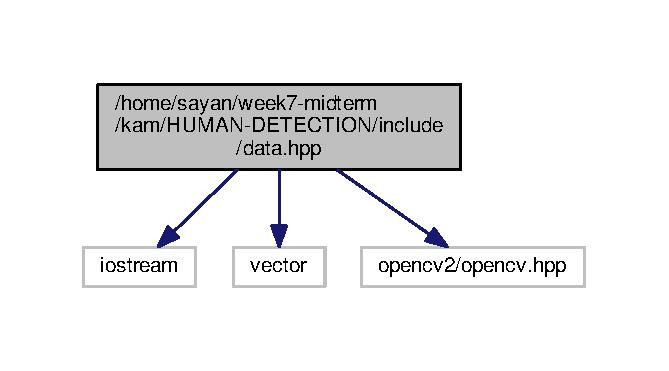
\includegraphics[width=321pt]{data_8hpp__incl}
\end{center}
\end{figure}
This graph shows which files directly or indirectly include this file\+:
\nopagebreak
\begin{figure}[H]
\begin{center}
\leavevmode
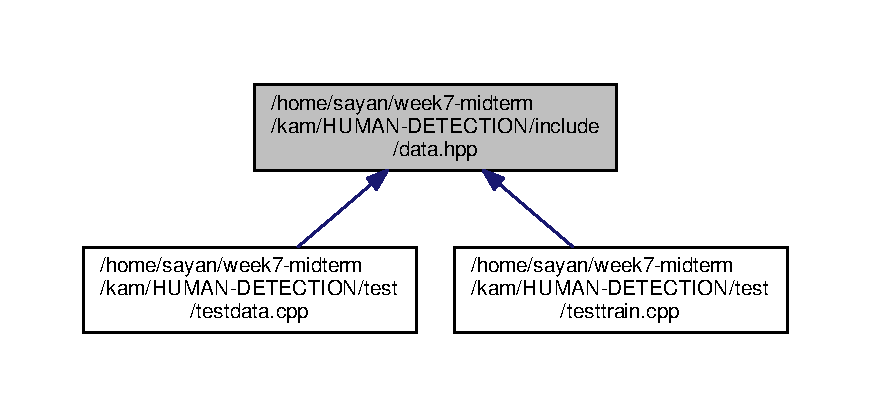
\includegraphics[width=350pt]{data_8hpp__dep__incl}
\end{center}
\end{figure}
\subsection*{Classes}
\begin{DoxyCompactItemize}
\item 
class \hyperlink{classData}{Data}
\end{DoxyCompactItemize}


\subsection{Detailed Description}
This is the stub for the \hyperlink{classData}{Data} class. 

\begin{DoxyAuthor}{Author}
kamakshi jain, Sayan Brahma
\end{DoxyAuthor}
\begin{DoxyCopyright}{Copyright}
\mbox{[}2019\mbox{]} kamakshi jain , Sayan Brahma 
\end{DoxyCopyright}

\hypertarget{detect_8hpp}{}\section{/home/sayan/week7-\/midterm/kam/\+H\+U\+M\+A\+N-\/\+D\+E\+T\+E\+C\+T\+I\+O\+N/include/detect.hpp File Reference}
\label{detect_8hpp}\index{/home/sayan/week7-\/midterm/kam/\+H\+U\+M\+A\+N-\/\+D\+E\+T\+E\+C\+T\+I\+O\+N/include/detect.\+hpp@{/home/sayan/week7-\/midterm/kam/\+H\+U\+M\+A\+N-\/\+D\+E\+T\+E\+C\+T\+I\+O\+N/include/detect.\+hpp}}


This is the stub for the \hyperlink{classDetect}{Detect} class.  


{\ttfamily \#include $<$iostream$>$}\\*
{\ttfamily \#include $<$vector$>$}\\*
{\ttfamily \#include $<$string$>$}\\*
{\ttfamily \#include $<$opencv2/opencv.\+hpp$>$}\\*
Include dependency graph for detect.\+hpp\+:
\nopagebreak
\begin{figure}[H]
\begin{center}
\leavevmode
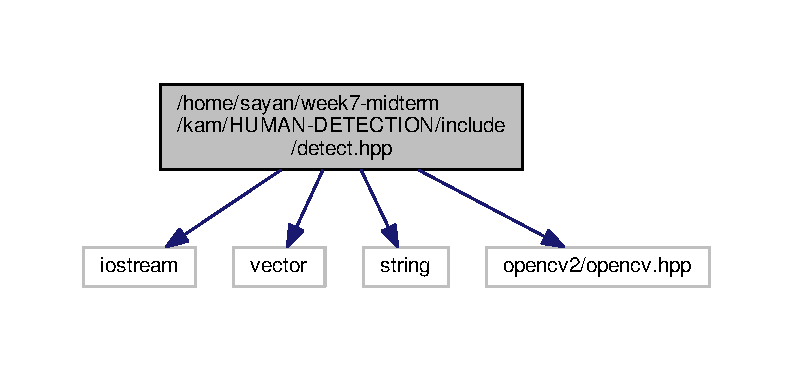
\includegraphics[width=350pt]{detect_8hpp__incl}
\end{center}
\end{figure}
\subsection*{Classes}
\begin{DoxyCompactItemize}
\item 
class \hyperlink{classDetect}{Detect}
\end{DoxyCompactItemize}


\subsection{Detailed Description}
This is the stub for the \hyperlink{classDetect}{Detect} class. 

\begin{DoxyAuthor}{Author}
kamakshi jain, Sayan Brahma
\end{DoxyAuthor}
\begin{DoxyCopyright}{Copyright}
\mbox{[}2019\mbox{]} kamakshi jain, Sayan Brahma 
\end{DoxyCopyright}

\hypertarget{train_8hpp}{}\section{/home/sayan/week7-\/midterm/kam/\+H\+U\+M\+A\+N-\/\+D\+E\+T\+E\+C\+T\+I\+O\+N/include/train.hpp File Reference}
\label{train_8hpp}\index{/home/sayan/week7-\/midterm/kam/\+H\+U\+M\+A\+N-\/\+D\+E\+T\+E\+C\+T\+I\+O\+N/include/train.\+hpp@{/home/sayan/week7-\/midterm/kam/\+H\+U\+M\+A\+N-\/\+D\+E\+T\+E\+C\+T\+I\+O\+N/include/train.\+hpp}}


This is the stub for the \hyperlink{classTrain}{Train} class.  


{\ttfamily \#include $<$iostream$>$}\\*
{\ttfamily \#include $<$vector$>$}\\*
{\ttfamily \#include $<$opencv2/opencv.\+hpp$>$}\\*
Include dependency graph for train.\+hpp\+:
\nopagebreak
\begin{figure}[H]
\begin{center}
\leavevmode
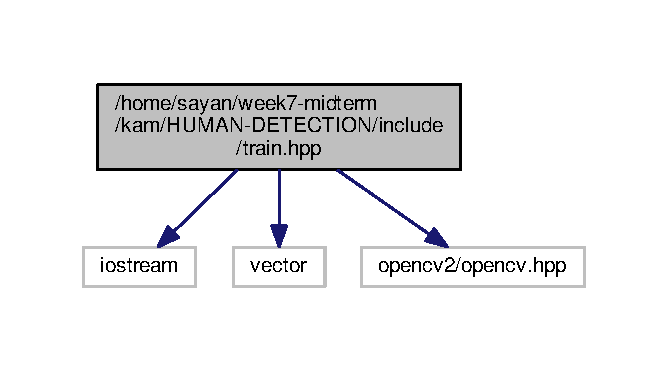
\includegraphics[width=321pt]{train_8hpp__incl}
\end{center}
\end{figure}
This graph shows which files directly or indirectly include this file\+:
\nopagebreak
\begin{figure}[H]
\begin{center}
\leavevmode
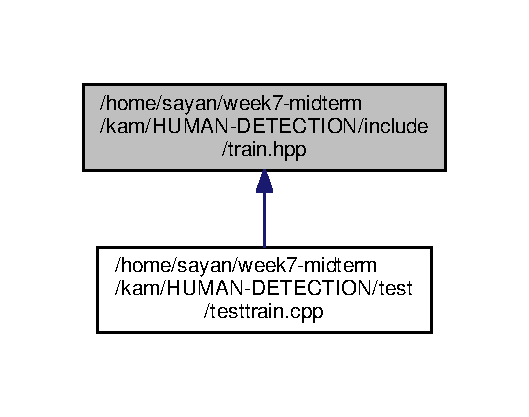
\includegraphics[width=254pt]{train_8hpp__dep__incl}
\end{center}
\end{figure}
\subsection*{Classes}
\begin{DoxyCompactItemize}
\item 
class \hyperlink{classTrain}{Train}
\end{DoxyCompactItemize}


\subsection{Detailed Description}
This is the stub for the \hyperlink{classTrain}{Train} class. 

\begin{DoxyAuthor}{Author}
kamakshi jain, Sayan Brahma
\end{DoxyAuthor}
\begin{DoxyCopyright}{Copyright}
\mbox{[}2019\mbox{]} kamakshi jain, Sayan Brahma 
\end{DoxyCopyright}

\hypertarget{testdata_8cpp}{}\section{/home/sayan/week7-\/midterm/kam/\+H\+U\+M\+A\+N-\/\+D\+E\+T\+E\+C\+T\+I\+O\+N/test/testdata.cpp File Reference}
\label{testdata_8cpp}\index{/home/sayan/week7-\/midterm/kam/\+H\+U\+M\+A\+N-\/\+D\+E\+T\+E\+C\+T\+I\+O\+N/test/testdata.\+cpp@{/home/sayan/week7-\/midterm/kam/\+H\+U\+M\+A\+N-\/\+D\+E\+T\+E\+C\+T\+I\+O\+N/test/testdata.\+cpp}}


This is the test for the data class.  


{\ttfamily \#include $<$gtest/gtest.\+h$>$}\\*
{\ttfamily \#include $<$data.\+hpp$>$}\\*
Include dependency graph for testdata.\+cpp\+:
\nopagebreak
\begin{figure}[H]
\begin{center}
\leavevmode
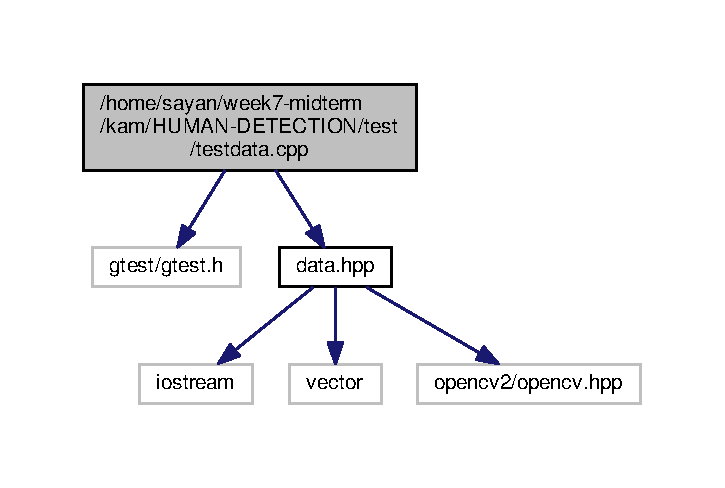
\includegraphics[width=348pt]{testdata_8cpp__incl}
\end{center}
\end{figure}
\subsection*{Functions}
\begin{DoxyCompactItemize}
\item 
{\bfseries T\+E\+ST} (Data\+Test, Data\+Load\+Pos\+Images\+Test)\hypertarget{testdata_8cpp_a4274370ed53aed7bb55ab4c5325dd8e8}{}\label{testdata_8cpp_a4274370ed53aed7bb55ab4c5325dd8e8}

\item 
{\bfseries T\+E\+ST} (Data\+Test, Data\+Load\+Neg\+Images\+Test)\hypertarget{testdata_8cpp_a9a98665fdafc850608daa8a521804624}{}\label{testdata_8cpp_a9a98665fdafc850608daa8a521804624}

\end{DoxyCompactItemize}


\subsection{Detailed Description}
This is the test for the data class. 

\begin{DoxyAuthor}{Author}
kamakshi jain, Sayan brahma
\end{DoxyAuthor}
\begin{DoxyCopyright}{Copyright}
\mbox{[}2019\mbox{]} kamakshi jain, Sayan brahma 
\end{DoxyCopyright}

\hypertarget{testtrain_8cpp}{}\section{test/testtrain.cpp File Reference}
\label{testtrain_8cpp}\index{test/testtrain.\+cpp@{test/testtrain.\+cpp}}


This is the test file to do test for train class.  


{\ttfamily \#include $<$gtest/gtest.\+h$>$}\\*
{\ttfamily \#include $<$data.\+hpp$>$}\\*
{\ttfamily \#include $<$train.\+hpp$>$}\\*
Include dependency graph for testtrain.\+cpp\+:
\nopagebreak
\begin{figure}[H]
\begin{center}
\leavevmode
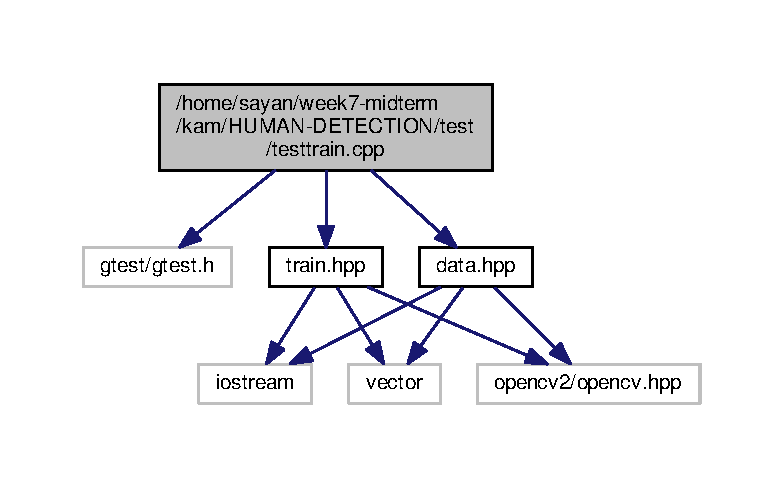
\includegraphics[width=350pt]{testtrain_8cpp__incl}
\end{center}
\end{figure}
\subsection*{Functions}
\begin{DoxyCompactItemize}
\item 
\hyperlink{testtrain_8cpp_af258a280e367e7ea70bedeed7076b958}{T\+E\+ST} (Train\+Test, Train\+Get\+H\+O\+G\+Test)
\item 
\hyperlink{testtrain_8cpp_ac55d451faf4ffbaee0822a7e2c2bd064}{T\+E\+ST} (Train\+Test, Train\+S\+V\+M\+Test)
\item 
\hyperlink{testtrain_8cpp_a644fb7dc805726eef5b8b7bc533f3700}{T\+E\+ST} (Train\+Test, Train\+Get\+Classifier\+Test)
\end{DoxyCompactItemize}


\subsection{Detailed Description}
This is the test file to do test for train class. 

M\+IT License

Copyright (c) 2019 Sayan Brahma, Kamakshi Jain

Permission is hereby granted, free of charge, to any person obtaining a copy of this software and associated documentation files (the \char`\"{}\+Software\char`\"{}), to deal in the Software without restriction, including without limitation the rights to use, copy, modify, merge, publish, distribute, sublicense, and/or sell copies of the Software, and to permit persons to whom the Software is furnished to do so, subject to the following conditions\+:

The above copyright notice and this permission notice shall be included in all copies or substantial portions of the Software.

T\+HE S\+O\+F\+T\+W\+A\+RE IS P\+R\+O\+V\+I\+D\+ED \char`\"{}\+A\+S I\+S\char`\"{}, W\+I\+T\+H\+O\+UT W\+A\+R\+R\+A\+N\+TY OF A\+NY K\+I\+ND, E\+X\+P\+R\+E\+SS OR I\+M\+P\+L\+I\+ED, I\+N\+C\+L\+U\+D\+I\+NG B\+UT N\+OT L\+I\+M\+I\+T\+ED TO T\+HE W\+A\+R\+R\+A\+N\+T\+I\+ES OF M\+E\+R\+C\+H\+A\+N\+T\+A\+B\+I\+L\+I\+TY, F\+I\+T\+N\+E\+SS F\+OR A P\+A\+R\+T\+I\+C\+U\+L\+AR P\+U\+R\+P\+O\+SE A\+ND N\+O\+N\+I\+N\+F\+R\+I\+N\+G\+E\+M\+E\+NT. IN NO E\+V\+E\+NT S\+H\+A\+LL T\+HE A\+U\+T\+H\+O\+RS OR C\+O\+P\+Y\+R\+I\+G\+HT H\+O\+L\+D\+E\+RS BE L\+I\+A\+B\+LE F\+OR A\+NY C\+L\+A\+IM, D\+A\+M\+A\+G\+ES OR O\+T\+H\+ER L\+I\+A\+B\+I\+L\+I\+TY, W\+H\+E\+T\+H\+ER IN AN A\+C\+T\+I\+ON OF C\+O\+N\+T\+R\+A\+CT, T\+O\+RT OR O\+T\+H\+E\+R\+W\+I\+SE, A\+R\+I\+S\+I\+NG F\+R\+OM, O\+UT OF OR IN C\+O\+N\+N\+E\+C\+T\+I\+ON W\+I\+TH T\+HE S\+O\+F\+T\+W\+A\+RE OR T\+HE U\+SE OR O\+T\+H\+ER D\+E\+A\+L\+I\+N\+GS IN T\+HE S\+O\+F\+T\+W\+A\+RE.

Copyright \mbox{[}2019\mbox{]} kamakshi jain, Sayan Brahma \begin{DoxyAuthor}{Author}
Kamakshi Jain, Sayan Brahma 
\end{DoxyAuthor}


\subsection{Function Documentation}
\index{testtrain.\+cpp@{testtrain.\+cpp}!T\+E\+ST@{T\+E\+ST}}
\index{T\+E\+ST@{T\+E\+ST}!testtrain.\+cpp@{testtrain.\+cpp}}
\subsubsection[{\texorpdfstring{T\+E\+S\+T(\+Train\+Test, Train\+Get\+H\+O\+G\+Test)}{TEST(TrainTest, TrainGetHOGTest)}}]{\setlength{\rightskip}{0pt plus 5cm}T\+E\+ST (
\begin{DoxyParamCaption}
\item[{Train\+Test}]{, }
\item[{Train\+Get\+H\+O\+G\+Test}]{}
\end{DoxyParamCaption}
)}\hypertarget{testtrain_8cpp_af258a280e367e7ea70bedeed7076b958}{}\label{testtrain_8cpp_af258a280e367e7ea70bedeed7076b958}
\index{testtrain.\+cpp@{testtrain.\+cpp}!T\+E\+ST@{T\+E\+ST}}
\index{T\+E\+ST@{T\+E\+ST}!testtrain.\+cpp@{testtrain.\+cpp}}
\subsubsection[{\texorpdfstring{T\+E\+S\+T(\+Train\+Test, Train\+S\+V\+M\+Test)}{TEST(TrainTest, TrainSVMTest)}}]{\setlength{\rightskip}{0pt plus 5cm}T\+E\+ST (
\begin{DoxyParamCaption}
\item[{Train\+Test}]{, }
\item[{Train\+S\+V\+M\+Test}]{}
\end{DoxyParamCaption}
)}\hypertarget{testtrain_8cpp_ac55d451faf4ffbaee0822a7e2c2bd064}{}\label{testtrain_8cpp_ac55d451faf4ffbaee0822a7e2c2bd064}
\index{testtrain.\+cpp@{testtrain.\+cpp}!T\+E\+ST@{T\+E\+ST}}
\index{T\+E\+ST@{T\+E\+ST}!testtrain.\+cpp@{testtrain.\+cpp}}
\subsubsection[{\texorpdfstring{T\+E\+S\+T(\+Train\+Test, Train\+Get\+Classifier\+Test)}{TEST(TrainTest, TrainGetClassifierTest)}}]{\setlength{\rightskip}{0pt plus 5cm}T\+E\+ST (
\begin{DoxyParamCaption}
\item[{Train\+Test}]{, }
\item[{Train\+Get\+Classifier\+Test}]{}
\end{DoxyParamCaption}
)}\hypertarget{testtrain_8cpp_a644fb7dc805726eef5b8b7bc533f3700}{}\label{testtrain_8cpp_a644fb7dc805726eef5b8b7bc533f3700}

%--- End generated contents ---

% Index
\backmatter
\newpage
\phantomsection
\clearemptydoublepage
\addcontentsline{toc}{chapter}{Index}
\printindex

\end{document}
